\documentclass[twocolumn, 9pt]{extarticle}
\usepackage{amsmath}
\usepackage{amssymb}
\usepackage{lineno,hyperref}
\usepackage[table,x11names,dvipsnames,table]{xcolor}
\usepackage{authblk}
\usepackage{natbib}
\usepackage{subcaption,booktabs}
\usepackage{graphicx}
\usepackage{multirow}
\usepackage[nolist,nohyperlinks]{acronym}
\usepackage{tabularx}
\usepackage{cleveref}
\usepackage{float}
\usepackage[group-separator={,}]{siunitx}
\usepackage{geometry}
 \geometry{
 a4paper,
 papersize={210mm,279mm},
 left=12.73mm,
 top=20.3mm,
 marginpar=3.53mm,
 textheight=238.4mm,
 right=12.73mm,
}

\setlength{\columnsep}{6.54mm}

\renewcommand{\familydefault}{\sfdefault}
\DeclareMathOperator*{\argmax}{arg\,max}
\DeclareMathOperator*{\argmin}{arg\,min}

\captionsetup[figure]{labelfont=bf,textfont=normalfont}
\captionsetup[subfigure]{labelfont=bf,textfont=normalfont}

\makeatletter
\def\@maketitle{
\raggedright
\newpage
  \noindent
  \vspace{0cm}
  \let \footnote \thanks
    {\hskip -0.4em \huge \textbf{{\@title}} \par}
    \vskip 1.5em
    {\large
      \lineskip .5em
      \begin{tabular}[t]{l}
      \raggedright
        \@author
      \end{tabular}\par}
    \vskip 1em
  \par
  \vskip 1.5em
  }
\makeatother

\bibliographystyle{abbrvnat}
\setcitestyle{authoryear,open={(},close={)}}

\begin{document}

\title{GUSTO Analysis}

\author{Matthew Lyon}

\date{}
\maketitle

\section{Introduction}

This is a report on the analysis of the GUSTO data.

\section{Initial Model Development} \label{sec:initial_model}

These experiments use only a small subset of CpG sites as a pilot study. Specifically, only 383 CpG sites are used within these experiments. Each subject has 4 timepoints: 3 months, 9 months, 42 months, and 72 months. In this setting, the 3, 9, and 42 months are used to predict the 72nd month. The data are split into training, validation, and test sets with an 80/10/10 split.

\subsection{Time-series Autoencoder}

This set of experiments uses an autoencoder structure, which consists of a CNN encoder, an LSTM layer, and a CNN decoder. The encoder and decoder use 1D convolutions across the feature (CpG site) space, and treat each timepoint independently. As information is passed through the encoder, the feature dimension is reduced. The LSTM layer then processes the reduced feature space across time. Finally, the decoder expands the feature space back to the original dimension. A learned time embedding is added to the input and output of the LSTM to encode the time (in months) into the data. The model had 240K trainable parameters, and the exact number of layers and hyperparameters are detailed in the code, specifically within \texttt{AutoEncoder} class within \texttt{gusto/experiments/cnn\_autoencoder/lib/autoencoder.py}.

\subsubsection{Experiments}
Below are the experiments that were run. The code for each experiment is located in the \texttt{gusto/experiments/cnn\_autoencoder} directory. The models are trained using an $\ell_{1}$ loss function, and results are reported in terms of the root mean squared error (RMSE) on the validation set. the optimiser AdamW is used with a learning rate of $0.001$. The training and validation losses for experiments 1, 2, and 3 are shown in \Cref{fig:losses_cnn}.

\paragraph{Experiment 1} The first experiment trains and validates the aforementioned model. The code for this experiment is located in \texttt{experiment\_1.py}. The experiments that follow are modifications of this experiment.

\paragraph{Experiment 2} This experiment uses the same model as Experiment 1, but applies a weighting to the input timepoints as a function of the distance (in time) from the target timepoint. The code for this experiment is located in \texttt{experiment\_2.py}. This modification did not improve the performance of the model.

\paragraph{Experiment 3} This experiment uses the same model as Experiment 1, but interpolates the time dimension of the data. This is done by using a continuously differentiable sub-spline built from piecewise cubic polynomials, known as Akima splines, and implemented in \href{https://docs.scipy.org/doc/scipy/reference/generated/scipy.interpolate.Akima1DInterpolator.html\#scipy.interpolate.Akima1DInterpolator}{scipy}. The data are then resampled using a perturbation in the time dimension of the original 3-, 9-, and 42-month timepoints. The perturbation is drawn from a Gaussian distribution with a mean of 0 and a standard deviation of 3 months. The code for this experiment is located in \texttt{experiment\_3.py}. The rationale behind this was to allow the model to learn a more continuous representation of the time dimension. This modification did not improve the performance of the model.

\begin{figure}
  \centering
  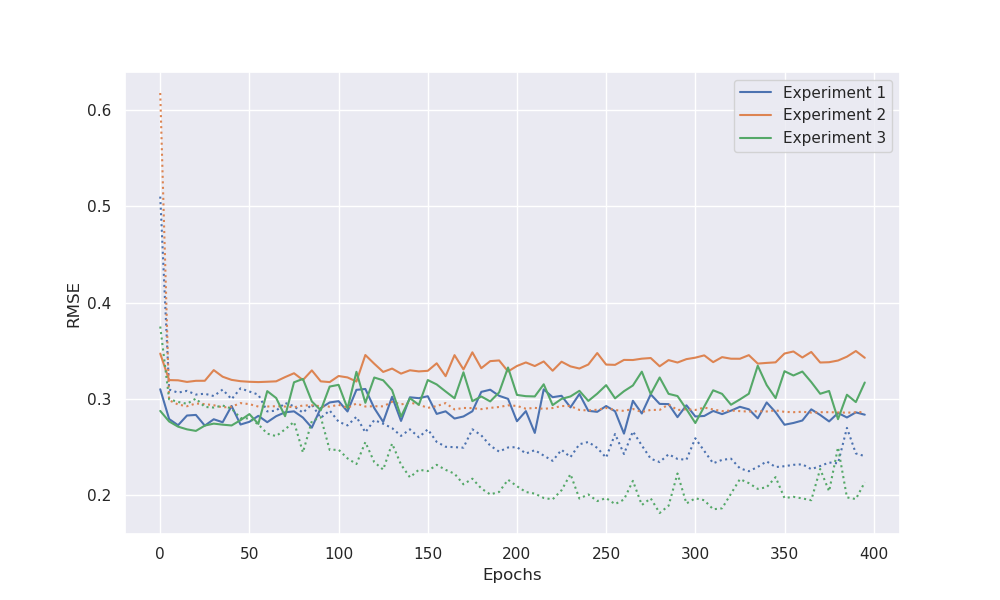
\includegraphics[width=\columnwidth]{cnn_autoencoder_experiments_1_to_3.png}
  \caption{Training and validation losses for experiments 1, 2, and 3. Dotted lines indicate the training loss, and solid lines indicate the validation loss.}
  \label{fig:losses_cnn}
\end{figure}

\paragraph{Experiment 4} This experiment consisted of a hyperparameter search over the number of layers, kernel sizes, latent dimension size, and use of batch normalisation, within the previous three experiments. The code for this experiment is located in \texttt{experiment\_4.py}. The best hyperparameters, as determined by the validation loss, for each of the three experiments were then used to train a model on the full dataset. The training and validation losses for each of the three experiments are shown in \Cref{fig:losses_cnn_hparams}. Overall, the hyperparameter search for each experiment did not yield a significant improvement in the model performance.

\begin{figure}
  \centering
  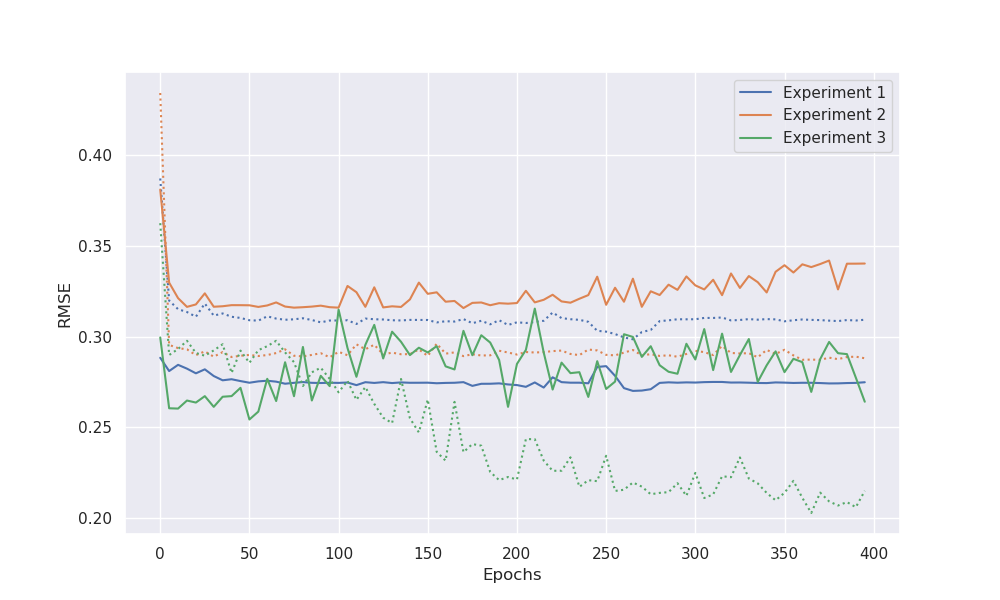
\includegraphics[width=\columnwidth]{cnn_autoencoder_experiments_4.png}
  \caption{Training and validation losses for experiments 1, 2, and 3 with hyperparameters determined via hyperparameter search. Dotted lines indicate the training loss, and solid lines indicate the validation loss.}
  \label{fig:losses_cnn_hparams}
\end{figure}

% \subsection{Independent CpG Sites}

% This set of experiments used a small multi-layer perceptron (MLP) to predict the 72 month timepoint from the 3, 9, and 42 month timepoints for independent CpG sites. The network had three hidden layers, each with 32 units, and used a ReLU activation function. The code for this experiment is located in \texttt{gusto/experiments/independent\_cpg}.

% Experiment 1 trains this model on the full training dataset as specified within \Cref{sec:initial_model}, whilst Experiment 2 trains the model on CpG sites that have no missing data. The rationale behind this was to determine if the model could learn a better representation of the data without missing values. The results of these experiments are shown in \Cref{fig:independent_cpg}.

\subsection{Dictionary Learning}

This set of experiments uses a dictionary learning approach as the encoder and decoder within the autoencoder, whilst using an LSTM to perform timeseries prediction in the latent space. Here, the data is arranged as $\mathbf{X} \in \mathbb{R}^{M \times N}$, where $N$ is the number of samples and $M$ is the number of features. In this case, the number of features is $M = 383$, and $N$ is the number of subjects multiplied by the number of timepoints. Dictionary learning supposes the data can be represented as a linear combination of a set of basis vectors, known as atoms. The atoms form a dictionary $\mathbf{D} \in \mathbb{R}^{M \times K}$ which is learned from the training data, and $K$ is the size of the latent space. The coefficients $\boldsymbol{\alpha} \in \mathbb{R}^{K \times N}$ of the linear combination are learnt jointly using a gradient descent procedure, where the dictionary and coefficients are updated in a two-step process:

\begin{equation}
  \argmin_{\mathbf{D}, \boldsymbol{\alpha}} \left\| \mathbf{X} - \mathbf{D} \boldsymbol{\alpha} \right\|_{2}^{2} + \lambda \left\| \boldsymbol{\alpha} \right\|_{1},
\end{equation}

\noindent where $\lambda$ is a sparsity parameter, and $\left\| \boldsymbol{\alpha} \right\|_{1}$ acts as a sparsity constraint on the coefficients. Once the dictionary and coefficients are learned, an LSTM $f_{\theta}$ is used to predict the output timepoint coefficients from the input timepoint coefficients:

\begin{equation}
  \argmin_{\theta} \left\| f_{\theta}(\boldsymbol{\alpha}^{(\mathrm{input})}) - \boldsymbol{\alpha}^{(\mathrm{output})} \right\|_{2}^{2},
\end{equation}

Training this model involves a three-step process:

\begin{enumerate}
  \item Train the dictionary $\mathbf{D}$ and coefficients $\boldsymbol{\alpha}_{\mathrm{train}}$ on the training dataset $\mathbf{X}_{\mathrm{train}}$. Here, $\mathbf{X}_{\mathrm{train}} = \left[ \mathbf{X}_{\mathrm{train}}^{(\mathrm{input})}\quad \mathbf{X}_{\mathrm{train}}^{(\mathrm{output})} \right]$ contains both the input timepoints, and the output timepoints, for each subject.
  \item Freeze the dictionary $\mathbf{D}$ and train $\boldsymbol{\alpha}_{\mathrm{validation}}^{(\mathrm{input})}$ corresponding to only the input timepoints within the validation dataset $\mathbf{X}_{\mathrm{validation}}^{(\mathrm{input})}$.
  \item Freeze the dictionary $\mathbf{D}$, $\boldsymbol{\alpha}_{\mathrm{train}}$, and $\boldsymbol{\alpha}_{\mathrm{validation}}^{(\mathrm{input})}$. Learn $f_{\theta}$ by predicting $\boldsymbol{\alpha}_{\mathrm{train}}^{(\mathrm{output})}$ from $\boldsymbol{\alpha}_{\mathrm{train}}^{(\mathrm{input})}$. Validate the model by predicting $\boldsymbol{\alpha}_{\mathrm{validation}}^{(\mathrm{output})}$ from $\boldsymbol{\alpha}_{\mathrm{validation}}^{(\mathrm{input})}$.
\end{enumerate}

\subsubsection{Experiments}

Below are the experiments that were run using the dictionary learning approach. The code for each experiment is located in the \texttt{gusto/experiments/dict\_learning} directory. The training loss and validation loss for each of the models is shown in \Cref{fig:losses_dict}.

\begin{figure}
  \centering
  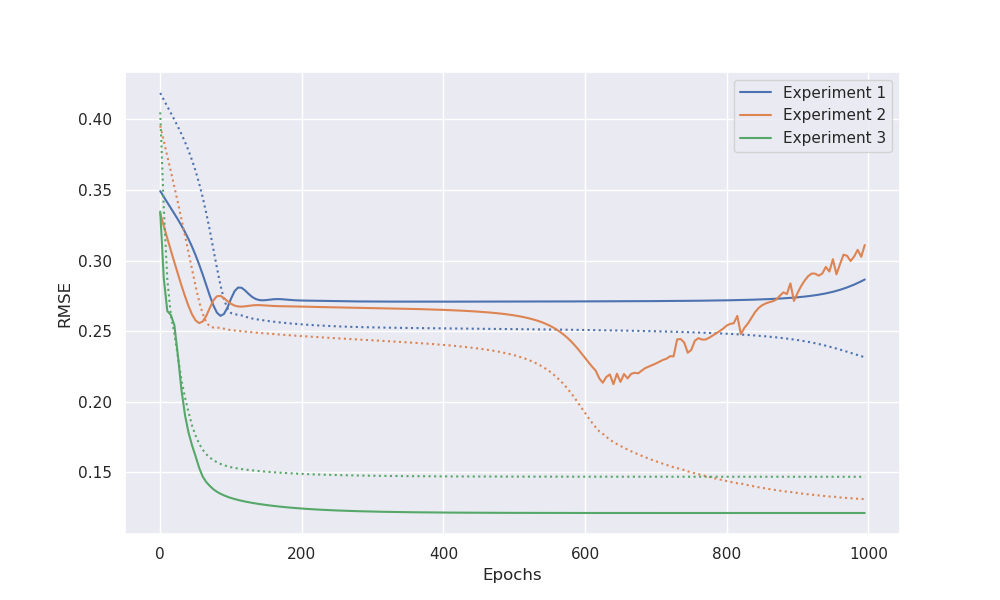
\includegraphics[width=\columnwidth]{dict_learning_experiments_1_to_3.png}
  \caption{Training and validation losses for experiments 1, 2, and 3. Dotted lines indicate the training loss, and solid lines indicate the validation loss.}
  \label{fig:losses_dict}
\end{figure}

\paragraph{Experiment 1} This experiment trains the dictionary learning model with a latent space size of 32, and $\lambda = 0.1$. The LSTM has 8.4K trainable parameters and the code for this experiment is located in \texttt{experiment\_1.py}.

\paragraph{Experiment 2} This experiment uses the same model as in Experiment 1, but with a dataset only consisting of examples with no missing data. Whilst the model performance was marginally better for most of the training, the model began to overfit around the 500 epoch mark. The code for this experiment is located in \texttt{experiment\_2.py}.

\paragraph{Experiment 3} This experiment uses a slightly higher parameter LSTM model, and adds a periodic time encoding to the input and output of the LSTM. Specifically, this time encoding is a sinusoidal projection of the time dimension, as described as the positional encoding in \cite{vaswani2017attention}. The number of trainable parameters within this LSTM is 10.5K. The code for this experiment is located in \texttt{experiment\_3.py}. This modification substantially improved performance, with a validation loss of around 0.1.

\paragraph{Experiment 4} Given the relative success of Experiment 3, this experiment plots the training and validation curves for varying latent space sizes using the same model. The code for this experiment is located in \texttt{experiment\_4.py}. The results of this experiment are shown in \Cref{fig:losses_dict_latent_space}.

\begin{figure}
  \centering
  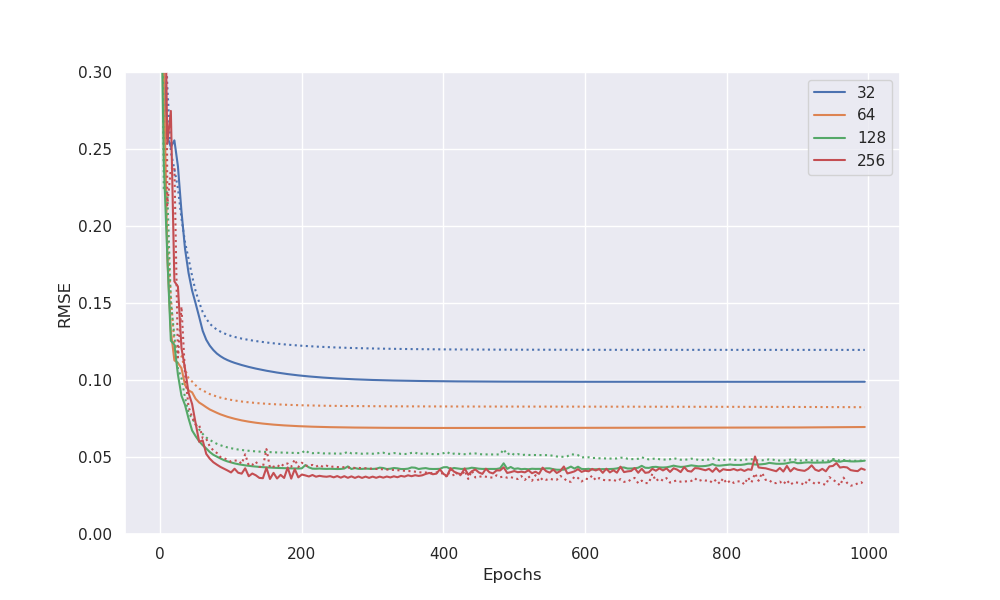
\includegraphics[width=\columnwidth]{dict_learning_experiments_4.png}
  \caption{Training and validation losses for the model proposed in Experiment 3, with varying latent space sizes. Dotted lines indicate the training loss, and solid lines indicate the validation loss.}
  \label{fig:losses_dict_latent_space}
\end{figure}

\section{Large Data Model Development}

This section details the development of a model using the full number of CpG sites available. At the time of writing, only the 3-month, 9-month, and 48-month timepoints are available. Thus, the 3- and 9-month timepoints are used to predict the 48-month timepoint. This dataset consists of 760,446 CpG sites and 172 subjects. The data are split into training and validation at a 90/10 split across subjects.

\subsection{U-Net}

This set of experiments uses a U-Net architecture to predict the 48-month timepoint from the 3- and 9-month timepoints. The U-Net architecture consists of an encoder and decoder, with skip connections between the encoder and decoder. The data is reshaped into a 2D image, with the channel dimension representing the timepoints, and the spatial dimensions representing the CpG sites. The encoder and decoder use 2D convolutions, and the model is trained using an $\ell_{1}$ loss function. The optimiser AdamW is used with a learning rate of $0.001$. The code for this experiment is located in the \texttt{gusto/experiments/unet} directory.

\subsubsection{Experiments}

Below are the experiments that were run using the U-Net architecture. The training and validation losses for each of the models are shown in \Cref{fig:losses_unet}, as well as a baseline training run using the dictionary learning method with a latent size of $128$ and regressing the 48-month timepoint from the 3- and 9-month timepoints.

\paragraph{Experiment 1} This experiment trains the U-Net model with hyperparameters and architecture as specified in \citet{ronneberger2015u}. Specifically, the model takes an input of size $2 \times 256 \times 256$, produces an output of size $1 \times 256 \times 256$, and has 7.8M trainable parameters. The 760,446 CpG sites are split into independent training examples of size $ 256 \times 256 = 65536$, where some sites are reused to produce a dataset size that is divisible by the image size. The code for this experiment is located in \texttt{experiment\_1.py}. The model was trained over multiple runs, for 50 epochs, and the best training and validation losses are shown in \Cref{fig:losses_unet}. The model achieved a validation loss of around $0.05$, which was lower than the dictionary learning baseline, despite the orders of magnitude increase in the number of CpG sites.

\paragraph{Experiment 2} This experiment uses the best-trained model from Experiment 1, and performs channel-wise pruning of 20\% and 40\% based on the $\ell_{1}$ norm of the weights. The rationale behind this was to perform a preliminary investigation of potential model compression techniques. The code for this experiment is located in \texttt{experiment\_2.py}. The results of the experiment show that pruning the model in both cases led to a small drop in validation performance compared to the unpruned model.

\begin{figure}
  \centering
  \includegraphics[width=\columnwidth]{unet_experiments_1_to_.png}
  \caption{Training and validation losses for the model proposed in Experiment 1 and 2. The curves shown are from training runs which yielded the lowest validation loss. Dotted lines indicate the training loss, and solid lines indicate the validation loss.}
  \label{fig:losses_unet}
\end{figure}

\begin{figure}
  \centering
  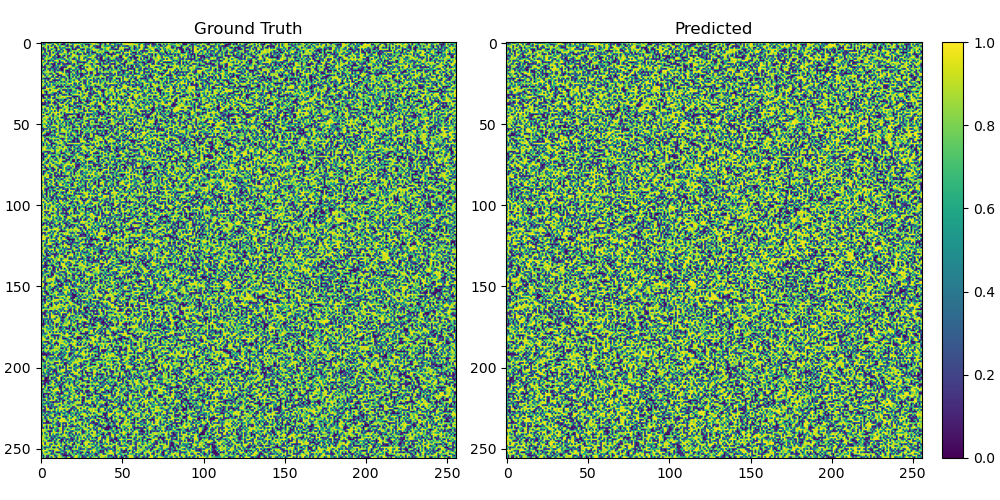
\includegraphics[width=\columnwidth]{unet_pred.png}
  \caption{Ground truth and predicted CpG sites for 48 months reshaped into an image. The predicted output is from the model trained in Experiment 1.}
  \label{fig:unet_pred}
\end{figure}

% \paragraph{Experiment 2} This experiment uses the same model as in Experiment 1, but with 4 input channels, where the additional channels are the 3- and 9-month CpG sites transformed via a Fourier transform into the frequency domain. The rationale behind this is that due to the random arrangement of CpG sites into a 2D image, much of the signal would be 

\bibliography{references}
\end{document}